\documentclass[conference,a4paper]{IEEEtran}
\usepackage[T1]{fontenc}
\usepackage[utf8]{inputenc}
\usepackage{babel}
\babelprovide[import,main]{indonesian}
\usepackage{graphicx,amsmath,booktabs,url,cite}
\hyphenation{de-tek-si}

\begin{document}
\renewcommand{\IEEEkeywordsname}{Kata Kunci}
\renewcommand{\abstractname}{Abstrak}
\title{Menguji Keterbatasan Objek Kecil Berkelompok pada YOLO:\\Studi Empiris pada VisDrone-DET}

\author{\IEEEauthorblockN{Elsa Aiziyah}
\IEEEauthorblockA{Magister Kecerdasan Artifisial, Universitas Gadjah Mada\\
elsaaiziyah@gmail.com}}
\maketitle

\begin{abstract}
Paper YOLO asli menyatakan bahwa satu sel grid hanya memprediksi dua kotak dan satu kelas, sehingga objek kecil yang berkelompok sulit dideteksi. Penelitian ini menguji klaim tersebut dalam tiga langkah pada VisDrone-DET. Pertama, penelitian ini menghitung fraksi objek yang kehilangan sel penanggung jawab pada formulasi YOLOv1. Kedua, penelitian ini mengukur AP gaya COCO menurut ukuran objek dan kepadatan citra pada YOLO11n, YOLO11s, dan YOLO11n hasil \textit{fine-tuning}. Ketiga, penelitian ini membandingkan intervensi resolusi masukan dan \textit{tiling}. Hasilnya, 74,0\% objek kehilangan sel pada grid $7\times7$. YOLO11 tetap lemah pada objek kecil (AP@0,5 0,171 untuk kecil dan 0,871 untuk besar pada masukan 640), tetapi kelemahan itu terutama berkaitan dengan resolusi efektif, bukan dengan batas satu objek per sel. Menaikkan resolusi masukan ke 1280 piksel menaikkan AP@0,5 objek kecil 1,6 sampai 2,1 kali dan memperkecil penurunan akibat kepadatan, sedangkan \textit{tiling} tidak mengungguli resolusi 1280 dan memerlukan waktu sekitar 2,6 sampai 3,8 kali lebih lama. Notebook Google Colab yang dapat dijalankan ulang tersedia di \url{TAUTAN-COLAB-DIISI-SEBELUM-DIKUMPULKAN}.
\end{abstract}

\begin{IEEEkeywords}
YOLO, deteksi objek kecil, VisDrone, \textit{tiling}, reproduktibilitas
\end{IEEEkeywords}

\section{Pendahuluan}
YOLO merumuskan deteksi objek sebagai satu regresi dari citra ke tensor $S\times S\times(5B+C)$, sehingga satu lintasan jaringan cukup untuk memprediksi seluruh objek pada citra \cite{redmon2016}. Pada Bagian 2.4, Redmon dkk. mengakui tiga keterbatasan. Pertama, setiap sel grid hanya memprediksi dua kotak dan satu kelas, sehingga jumlah objek berdekatan yang dapat diprediksi terbatas dan objek kecil yang muncul berkelompok sulit dideteksi. Kedua, fitur yang dipakai untuk memprediksi kotak tergolong kasar akibat banyaknya \textit{downsampling}. Ketiga, fungsi \textit{loss} memperlakukan galat pada kotak kecil sama dengan galat pada kotak besar.

YOLO modern telah mengubah banyak komponen tersebut. YOLO11 \cite{jocher2024} memakai \textit{neck} piramida fitur multiskala \cite{lin2017fpn}, kepala deteksi tanpa \textit{anchor}, penetapan target selaras tugas \cite{feng2021tood}, dan \textit{distribution focal loss} \cite{li2020gfl}. Pertanyaan yang muncul adalah apakah keterbatasan pada objek kecil yang berkelompok masih berlaku pada YOLO modern.

VisDrone-DET \cite{du2019visdrone} menjadi himpunan data uji yang sesuai karena memuat citra drone dengan objek yang sangat kecil dan padat. Pada set \textit{val}, 68,6\% objek berukuran kecil (luas kurang dari $32^2$ piksel), median kepadatan mencapai 65 objek per citra, dan 65,5\% citra memuat lebih dari 49 objek, yaitu kapasitas maksimum grid $7\times7$ pada YOLOv1.

Penelitian ini menjawab tiga pertanyaan riset yang dapat diuji secara empiris.
\begin{enumerate}
\item \textbf{RQ1.} Berapa fraksi objek VisDrone yang kehilangan sel penanggung jawab pada formulasi YOLOv1, dan bagaimana fraksi itu berubah pada grid yang lebih rapat?
\item \textbf{RQ2.} Apakah YOLO11 masih lebih lemah pada objek kecil dan pada citra yang padat, bila diukur dengan AP@0,5 dan AP@0,5:0,95 menurut ukuran objek?
\item \textbf{RQ3.} Apakah menaikkan resolusi masukan atau mengiris citra (\textit{tiling}) mengecilkan kesenjangan tersebut?
\end{enumerate}

\section{Metode}
\subsection{Ringkasan YOLOv1 dan klaim yang diuji}
YOLOv1 membagi citra menjadi grid $S\times S$ dengan $S=7$. Sel yang memuat pusat objek bertanggung jawab memprediksi objek itu. Bila $(c_x,c_y)$ adalah pusat kotak yang dinormalisasi terhadap citra, sel penanggung jawab berada pada baris $i$ dan kolom $j$ dengan
\begin{equation}
j=\lfloor c_x S\rfloor,\quad i=\lfloor c_y S\rfloor,\quad x=c_x S-j,\quad y=c_y S-i,
\label{eq:target}
\end{equation}
sedangkan $w$ dan $h$ dinormalisasi terhadap citra. Setiap sel memprediksi $B=2$ kotak $(x,y,w,h,\text{kepercayaan})$ dan satu himpunan probabilitas kelas $C$, sehingga satu sel hanya dapat membawa satu objek. Fungsi \textit{loss} menggunakan $\sqrt{w}$ dan $\sqrt{h}$ untuk meredam perbedaan galat antara kotak kecil dan besar, tetapi paper mengakui bahwa pendekatan ini hanya mengurangi masalahnya.

\subsection{Bagian yang diimplementasikan}
Implementasi mencakup empat komponen yang dikerjakan sendiri. Pertama, fungsi \texttt{encode\_yolov1\_target} menerapkan Persamaan~\eqref{eq:target} dan menghitung objek yang kehilangan sel (RQ1). Kedua, evaluator AP gaya COCO memakai antarmuka \texttt{pycocotools} (dengan implementasi \texttt{faster-coco-eval} bila tersedia) dengan rincian ukuran dan kepadatan serta wilayah abaikan VisDrone. Ketiga, fungsi inferensi mencakup resolusi masukan dan \textit{tiling} beserta penggabungan NMS (RQ3). Keempat, analisis sensitivitas IoU dan resolusi efektif menguji klaim tentang galat kotak kecil. Detektor YOLO11 dipakai melalui pustaka Ultralytics dan tidak ditulis ulang dari awal.

\subsection{Perbedaan dengan paper dan alasannya}
Penelitian ini tidak melatih ulang YOLOv1 karena tujuan yang diuji adalah apakah keterbatasannya masih berlaku pada detektor modern. Analisis struktural YOLOv1 dilakukan lewat penetapan target tanpa melatih jaringan, sehingga hasilnya berupa batas atas recall dan bukan performa terukur. YOLO11 menetapkan target secara banyak-ke-satu pada tiga skala (stride 8, 16, dan 32), sehingga batas satu objek per sel tidak berlaku. Karena itu hasil RQ1 untuk $S>7$ menunjukkan seberapa ketat batas tersebut bila diterapkan pada grid rapat, dan tidak menggambarkan YOLO11. Paper melaporkan mAP pada PASCAL VOC, sedangkan penelitian ini memakai VisDrone-DET, sehingga angka mutlaknya tidak sebanding.

\section{Setup Eksperimen}
\subsection{Data}
Himpunan data adalah VisDrone-DET 2019 \cite{du2019visdrone} dengan sepuluh kelas (\textit{pedestrian, people, bicycle, car, van, truck, tricycle, awning-tricycle, bus, motor}). Set uji adalah seluruh \textit{val} (548 citra, 38.759 objek). Pelatihan memakai subset \textit{train} yang dipilih acak dengan seed 42, yaitu 1.000 citra untuk pelatihan dan 50 citra \textit{hold-out} untuk pemilihan \textit{checkpoint}, sehingga set uji tidak disentuh selama pelatihan. Anotasi berskor 0 (wilayah diabaikan dan kategori \textit{others}) diperlakukan sebagai wilayah abaikan.

\subsection{Model dan intervensi}
Tiga model dibandingkan, yaitu YOLO11n pralatih COCO (\textit{zero-shot}), YOLO11s pralatih COCO sebagai pembanding kapasitas, dan YOLO11n hasil \textit{fine-tuning} pada subset VisDrone. Model \textit{zero-shot} hanya memakai kelas COCO yang berpadanan (\textit{person, bicycle, car, motorcycle, bus, truck}). Lima konfigurasi inferensi diuji: masukan 640, 960, dan 1280 piksel, \textit{tiling} (irisan $640\times640$ dengan tumpang tindih 20\% pada resolusi asli, digabung NMS IoU 0,5), dan \textit{tiling} ditambah satu inferensi citra penuh. Teknik \textit{tiling} ini disederhanakan dari SAHI \cite{akyon2022sahi}. Pada seluruh konfigurasi, ambang kepercayaan 0,001, NMS agnostik kelas dengan IoU 0,7, dan maksimum 500 deteksi digunakan.

\subsection{Metrik}
Metrik utama adalah AP@0,5 dan AP@0,5:0,95 gaya COCO \cite{lin2014coco} yang dirinci menurut ukuran objek: kecil ($<32^2$ piksel), sedang ($32^2$ sampai $96^2$), dan besar ($>96^2$) pada resolusi asli. Batas deteksi per citra dinaikkan dari 100 menjadi 500, karena citra \textit{val} memuat hingga 317 objek. Mode agnostik kelas dipakai agar model \textit{zero-shot} dan \textit{fine-tuned} dapat dibandingkan, dan mAP sadar kelas (10 kelas) dilaporkan khusus bagi model \textit{fine-tuned}. Pengujian mandiri evaluator (GT sebagai deteksi) menghasilkan AP mendekati 1. Kepadatan citra dibagi menjadi tiga kelompok berdasarkan tersil jumlah objek per citra.

\subsection{Komputasi}
Seluruh eksperimen berjalan di Google Colab dengan GPU NVIDIA Tesla T4 dan 2 inti CPU, memakai Python 3.13.15, PyTorch 2.11.0+cu130, dan Ultralytics 8.4.172. Seed acak adalah 42. Notebook dapat dijalankan ulang di Google Colab dari awal sampai akhir.


\section{Hasil}
\subsection{Batas struktural satu objek per sel (RQ1)}
Tabel~\ref{tab:grid} menunjukkan bahwa pada grid $7\times7$ milik YOLOv1, hanya 26,0\% objek yang dapat ditetapkan ke sel yang bertanggung jawab, sehingga 74,0\% objek kehilangan sel. Fraksi itu turun menjadi 40,3\% pada $S=20$ (setara stride 32 pada masukan 640) dan 2,0\% pada $S=160$. Angka ini merupakan batas atas recall struktural, bukan performa terukur dari jaringan.

\begin{table}[t]
\caption{Fraksi objek VisDrone-DET \textit{val} yang kehilangan sel penanggung jawab bila satu sel hanya memuat satu objek.}
\label{tab:grid}
\centering\scriptsize
\begin{tabular}{rrlr}
\toprule
$S$ & Sel & Padanan & Hilang (\%) \\
\midrule
7 & 49 & YOLOv1 (paper) & 74,0 \\
13 & 169 & stride 32 \,@\, $\sim$416 & 55,0 \\
20 & 400 & stride 32 \,@\, 640 & 40,3 \\
40 & 1600 & stride 16 \,@\, 640 & 20,4 \\
80 & 6400 & stride 8 \,@\, 640 & 7,8 \\
160 & 25600 & stride 8 \,@\, 1280 & 2,0 \\
\bottomrule
\end{tabular}
\end{table}


\begin{figure}[t]
\centering
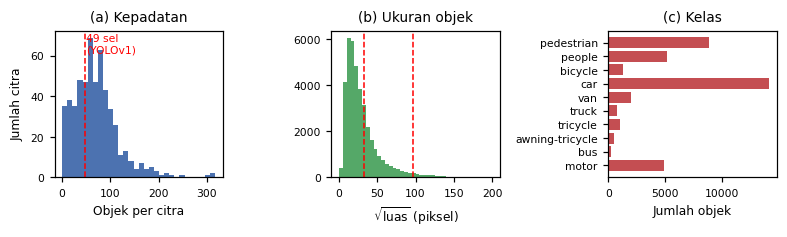
\includegraphics[width=\columnwidth]{g1_statistik.png}
\caption{Statistik set \textit{val} VisDrone-DET: (a) jumlah objek per citra dengan batas 49 sel milik YOLOv1, (b) ukuran objek ($\sqrt{\text{luas}}$) dengan batas 32 dan 96 piksel, dan (c) jumlah objek per kelas.}
\label{fig:data}
\end{figure}

\subsection{Kinerja menurut ukuran objek (RQ2)}
Tabel~\ref{tab:utama} merangkum kinerja seluruh konfigurasi dan Gambar~\ref{fig:ukuran} menampilkan AP@0,5 menurut ukuran. Pada masukan 640, YOLO11n \textit{zero-shot} mencapai AP@0,5 0,171 untuk objek kecil dan 0,871 untuk objek besar, yaitu selisih 5,1 kali. Setelah \textit{fine-tuning}, nilainya menjadi 0,290 dan 0,947, yaitu selisih 3,3 kali. Rasio AP@0,5:0,95 terhadap AP@0,5 pada model \textit{fine-tuned} adalah 0,37 untuk objek kecil dan 0,82 untuk objek besar. Pada model \textit{zero-shot} (640), rasio yang sama adalah 0,36 dan 0,79. Pada resolusi 640, 30,8\% objek berukuran kurang dari 8 piksel dan 69,9\% kurang dari 16 piksel; pada 1280, angkanya 5,7\% dan 30,8\%. Pergeseran dua piksel menurunkan IoU kotak 8 piksel menjadi 0,600, sedangkan pada kotak 64 piksel IoU tetap 0,939.

\begin{table*}[t]
\caption{AP@0,5 dan AP@0,5:0,95 (agnostik kelas) menurut ukuran objek pada 548 citra VisDrone-DET \textit{val}. K = kecil, S = sedang, B = besar, A = semua ukuran. AR@0,5 adalah \textit{recall} objek kecil tanpa ambang skor. Waktu diukur pada GPU Tesla T4 dan mencakup pembacaan citra.}
\label{tab:utama}
\centering\scriptsize
\begin{tabular}{llcccccccc}
\toprule
 & & \multicolumn{4}{c}{AP@0,5} & \multicolumn{2}{c}{AP@0,5:0,95} & AR@0,5 & \\
\cmidrule(lr){3-6}\cmidrule(lr){7-8}
Model & Konfigurasi & K & S & B & A & K & A & K & ms/citra \\
\midrule
YOLO11n \textit{zero-shot} & 640 & 0,171 & 0,583 & 0,871 & 0,304 & 0,061 & 0,157 & 0,297 & 17,8 \\
 & 960 & 0,288 & 0,679 & 0,895 & 0,418 & 0,115 & 0,225 & 0,484 & 18,6 \\
 & 1280 & 0,362 & 0,728 & 0,894 & 0,488 & 0,159 & 0,270 & 0,589 & 22,4 \\
 & \textit{tiling} & 0,341 & 0,696 & 0,857 & 0,464 & 0,141 & 0,242 & 0,576 & 85,4 \\
 & \textit{\textit{tiling}}+penuh & 0,336 & 0,690 & 0,874 & 0,457 & 0,138 & 0,239 & 0,573 & 103,8 \\
\midrule
YOLO11s \textit{zero-shot} & 640 & 0,256 & 0,679 & 0,917 & 0,397 & 0,100 & 0,214 & 0,402 & 18,2 \\
 & 1280 & 0,448 & 0,780 & 0,938 & 0,565 & 0,203 & 0,322 & 0,661 & 37,8 \\
 & \textit{tiling} & 0,410 & 0,736 & 0,886 & 0,526 & 0,175 & 0,286 & 0,642 & 98,3 \\
\midrule
YOLO11n \textit{fine-tuned} & 640 & 0,290 & 0,760 & 0,947 & 0,455 & 0,108 & 0,238 & 0,526 & 18,6 \\
 & 960 & 0,415 & 0,810 & 0,936 & 0,555 & 0,171 & 0,300 & 0,679 & 19,2 \\
 & 1280 & 0,471 & 0,811 & 0,901 & 0,591 & 0,200 & 0,321 & 0,745 & 22,6 \\
 & \textit{tiling} & 0,462 & 0,786 & 0,873 & 0,573 & 0,190 & 0,299 & 0,715 & 86,4 \\
 & \textit{\textit{tiling}}+penuh & 0,451 & 0,794 & 0,915 & 0,570 & 0,185 & 0,299 & 0,718 & 109,4 \\
\bottomrule
\end{tabular}
\end{table*}


\begin{figure}[t]
\centering
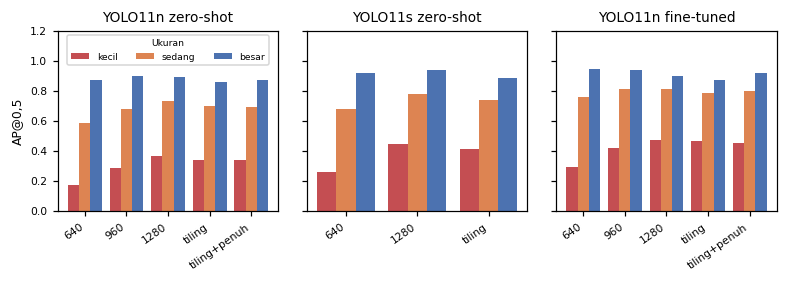
\includegraphics[width=\columnwidth]{g4_ap_ukuran.png}
\caption{AP@0,5 menurut ukuran objek untuk setiap model dan konfigurasi.}
\label{fig:ukuran}
\end{figure}

\subsection{Pengaruh kepadatan citra (RQ2)}
Set \textit{val} dibagi menjadi tiga kelompok dengan batas tersil 48 dan 83 objek per citra (184, 181, dan 183 citra). Pada model \textit{fine-tuned} dengan masukan 640, AP@0,5 objek kecil turun dari 0,338 (jarang) ke 0,270 (padat), yaitu 20,1\%. Pada model \textit{zero-shot}, penurunannya 21,5\% (0,209 ke 0,164). Pada masukan 1280, penurunan model \textit{fine-tuned} menjadi 6,9\% (0,496 ke 0,462) dan penurunan model \textit{zero-shot} menjadi 13,3\% (0,407 ke 0,353). Pada \textit{tiling}, penurunan model \textit{fine-tuned} 1,1\% (0,467 ke 0,462) dan penurunan model \textit{zero-shot} 6,0\% (0,364 ke 0,342). Tabel~\ref{tab:kepadatan} dan Gambar~\ref{fig:padat} merinci hasil ini.

\begin{table}[t]
\caption{AP@0,5 objek kecil menurut kepadatan citra (tersil jumlah objek per citra).}
\label{tab:kepadatan}
\centering\scriptsize
\begin{tabular}{llccc}
\toprule
Model & Konfigurasi & Jarang & Sedang & Padat \\
\midrule
YOLO11n \textit{zero-shot} & 640 & 0,209 & 0,181 & 0,164 \\
YOLO11n \textit{zero-shot} & \textit{tiling} & 0,364 & 0,343 & 0,342 \\
YOLO11s \textit{zero-shot} & 640 & 0,312 & 0,270 & 0,243 \\
YOLO11s \textit{zero-shot} & \textit{tiling} & 0,452 & 0,414 & 0,411 \\
YOLO11n \textit{fine-tuned} & 640 & 0,338 & 0,315 & 0,270 \\
YOLO11n \textit{fine-tuned} & \textit{tiling} & 0,467 & 0,460 & 0,462 \\
\bottomrule
\end{tabular}
\end{table}


\begin{figure}[t]
\centering
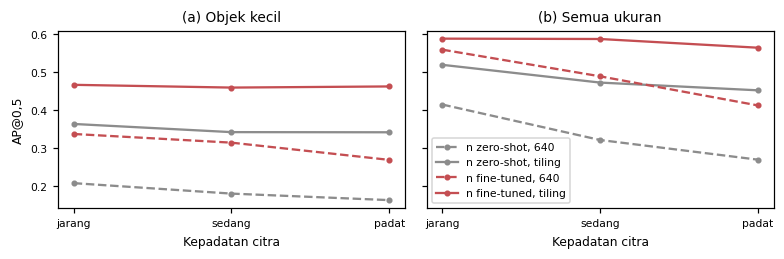
\includegraphics[width=\columnwidth]{g5_kepadatan.png}
\caption{AP@0,5 menurut kepadatan citra: (a) objek kecil dan (b) semua ukuran. Garis putus-putus adalah masukan 640 dan garis utuh adalah \textit{tiling}.}
\label{fig:padat}
\end{figure}

\subsection{Intervensi resolusi dan \textit{tiling} (RQ3)}
Menaikkan masukan dari 640 ke 1280 meningkatkan AP@0,5 objek kecil dari 0,171 ke 0,362 pada YOLO11n \textit{zero-shot} dan dari 0,290 ke 0,471 pada model \textit{fine-tuned}, dengan waktu per citra naik dari sekitar 18 ke 22 milidetik. \textit{Tiling} mencapai 0,341 dan 0,462 pada objek kecil dengan waktu sekitar 85 dan 86 milidetik. Dengan demikian, pada YOLO11n \textit{zero-shot}, YOLO11n \textit{fine-tuned}, dan YOLO11s \textit{zero-shot} (0,410 terhadap 0,448 pada objek kecil), \textit{tiling} tidak mengungguli resolusi 1280. Pada model \textit{fine-tuned}, \textit{tiling} menurunkan AP@0,5 objek besar dari 0,947 (640) menjadi 0,873, sedangkan penambahan inferensi citra penuh memulihkannya ke 0,915 dengan waktu 109 milidetik. Pada perbandingan kapasitas, YOLO11s pada 640 mencapai AP@0,5 objek kecil 0,256, lebih tinggi daripada YOLO11n pada 640 (0,171) tetapi lebih rendah daripada YOLO11n pada 960 (0,288). Pada mAP sadar kelas (Tabel~\ref{tab:map10}), model \textit{fine-tuned} mencapai 0,132 pada 640 dan 0,176 pada 1280; mAP@0,5 objek besar turun dari 0,293 ke 0,200 pada kenaikan resolusi tersebut.

\begin{table}[t]
\caption{mAP sadar kelas (10 kelas VisDrone) model YOLO11n \textit{fine-tuned}.}
\label{tab:map10}
\centering\scriptsize
\begin{tabular}{lccccc}
\toprule
 & \multicolumn{4}{c}{mAP@0,5} & mAP@0,5:0,95 \\
\cmidrule(lr){2-5}\cmidrule(lr){6-6}
Konfigurasi & K & S & B & A & A \\
\midrule
640 & 0,072 & 0,212 & 0,293 & 0,132 & 0,075 \\
960 & 0,112 & 0,244 & 0,267 & 0,168 & 0,096 \\
1280 & 0,135 & 0,244 & 0,200 & 0,176 & 0,099 \\
\textit{tiling} & 0,137 & 0,229 & 0,157 & 0,169 & 0,091 \\
\textit{\textit{tiling}}+penuh & 0,132 & 0,240 & 0,242 & 0,171 & 0,093 \\
\bottomrule
\end{tabular}
\end{table}


\section{Analisis}
\subsection{Apa yang didukung dan apa yang tidak}
\textbf{Klaim tentang grid didukung untuk YOLOv1, tetapi tidak menjelaskan YOLO11.} Hasil RQ1 menegaskan bahwa formulasi satu objek per sel pada $7\times7$ tidak dapat mencakup 74,0\% objek VisDrone. Namun YOLO11 menetapkan target banyak-ke-satu pada tiga skala, sehingga batas itu tidak berlaku. Bukti yang tersedia justru menunjuk resolusi efektif sebagai penyebab dominan: menaikkan resolusi pada arsitektur yang sama meningkatkan AP@0,5 objek kecil 1,6 sampai 2,1 kali, dan penurunan akibat kepadatan pada model \textit{fine-tuned} menyusut dari 20,1\% menjadi 6,9\% pada 1280 dan 1,1\% pada \textit{tiling}. Penurunan itu belum hilang sepenuhnya, misalnya 13,3\% pada model \textit{zero-shot} dengan masukan 1280, sehingga kepadatan tetap berpengaruh. Interpretasinya, pada 640 piksel sebagian besar objek (69,9\%) berukuran kurang dari 16 piksel, sehingga objek berdekatan diduga tergabung dalam satu sel fitur, dan menaikkan resolusi memisahkannya. Hubungan ini bersifat korelasional karena penelitian ini tidak memvariasikan stride secara terpisah.

\textbf{Klaim tentang galat kotak kecil didukung.} Rasio AP@0,5:0,95 terhadap AP@0,5 untuk objek kecil (0,37) jauh lebih rendah daripada objek besar (0,82), dan analisis sensitivitas menunjukkan bahwa pergeseran dua piksel saja menurunkan IoU kotak 8 piksel menjadi 0,600. Penyimpangan lokalisasi kecil sudah cukup menggagalkan kecocokan pada ambang IoU tinggi. Namun, bukti ini tidak memisahkan peran fungsi \textit{loss} dari peran diskretisasi piksel.

\subsection{Mengapa \textit{tiling} tidak mengungguli resolusi 1280}
Skala efektif kedua intervensi hampir sama (median sisi objek 22,8 piksel pada \textit{tiling} dan 22,5 piksel pada 1280), tetapi \textit{tiling} lebih lambat, lebih rendah pada seluruh model, dan menurunkan AP objek besar. Hipotesis yang sesuai dengan pola ini adalah objek yang terpotong di tepi irisan dan hilangnya konteks, dan bahwa penggabungan NMS mempertahankan potongan kotak yang tidak utuh. Pemulihan sebagian pada varian \textit{tiling}+penuh mendukung hipotesis konteks untuk objek besar. Hipotesis ini belum diuji langsung. Satu keunggulan \textit{tiling} adalah penurunan akibat kepadatan yang paling kecil (1,1\% pada model \textit{fine-tuned} dan 6,0\% pada model \textit{zero-shot}). Implementasi \textit{tiling} penelitian ini disederhanakan dari SAHI \cite{akyon2022sahi}, yaitu memakai irisan 640 piksel pada resolusi asli dengan tumpang tindih 20\% dan tidak melatih ulang dengan irisan.

\subsection{Kasus gagal}
Gambar~\ref{fig:gagal} memperlihatkan citra padat (persentil ke-90) dengan 122 objek valid. Model \textit{fine-tuned} menemukan 36 objek pada masukan 640 dan 43 objek pada \textit{tiling} (pada skor 0,25), sehingga recall pada citra ini naik dari 0,295 menjadi 0,352. Objek yang terlewat terkonsentrasi pada tiga tempat, yaitu kendaraan dan pejalan kaki kecil di jalan yang jauh, kerumunan pengendara motor di sisi kanan, dan kendaraan yang sebagian tertutup pohon di sisi kiri. Pada kerumunan itu, kotak GT saling bertumpuk, dan beberapa kotak kuning (positif palsu) tampak menutupi beberapa objek sekaligus, yaitu gejala penggabungan objek berdekatan pada satu keluaran. \textit{Tiling} mengurangi positif palsu dari 24 menjadi 18, tetapi 79 objek (64,8\%) tetap terlewat. Pada tingkat dataset dan ambang skor 0,25, \textit{tiling} menaikkan recall objek kecil dari 0,217 menjadi 0,404, tetapi menurunkan recall objek besar dari 0,90 menjadi 0,85. Citra ini menunjukkan batas intervensi, karena sebagian besar objek tetap terlewat meskipun dengan \textit{tiling}.

\begin{figure*}[t]
\centering
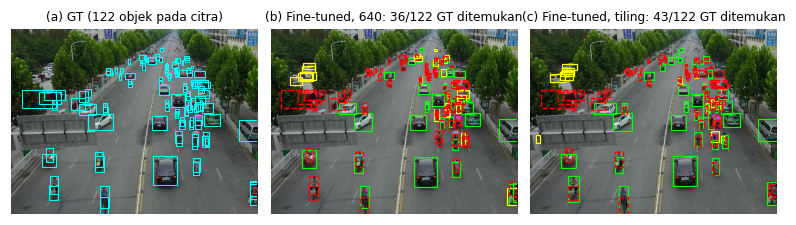
\includegraphics[width=\textwidth]{g6_kasus_gagal.png}
\caption{Kasus gagal pada citra padat: (a) GT, (b) hasil \textit{fine-tuned} pada masukan 640, dan (c) hasil \textit{tiling}. Hijau: deteksi benar; kuning: positif palsu; merah putus-putus: objek yang terlewat. Hanya deteksi berskor $\ge$ 0,25 yang ditampilkan.}
\label{fig:gagal}
\end{figure*}

\subsection{Hasil yang tidak sesuai harapan}
Dua hasil patut dicatat. Pertama, pada model \textit{fine-tuned}, AP objek besar justru turun saat resolusi naik (0,947 pada 640 menjadi 0,901 pada 1280). Model itu dilatih pada 640 piksel, sehingga objek besar pada 1280 melampaui skala yang pernah dilihat saat pelatihan. Ini dugaan yang belum diuji. Kedua, mAP sadar kelas tergolong rendah (0,132 sampai 0,176), konsisten dengan mAP@0,5 pada citra \textit{hold-out} sebesar 0,176 pada \textit{epoch} terakhir. Angka itu mencerminkan pelatihan yang singkat, yaitu 12 \textit{epoch} pada 1.000 citra.

\section{Kesimpulan dan Keterbatasan}
Penelitian ini menyimpulkan bahwa keterbatasan objek kecil berkelompok tetap terlihat pada YOLO11, tetapi penyebab utamanya adalah resolusi efektif, bukan batas satu objek per sel. Jawaban atas ketiga pertanyaan adalah sebagai berikut. RQ1: 74,0\% objek VisDrone kehilangan sel pada $S=7$ dan 2,0\% pada $S=160$. RQ2: AP@0,5 objek kecil tetap jauh di bawah objek besar (0,290 terhadap 0,947 pada model \textit{fine-tuned}), dan kepadatan menurunkannya 20,1\% pada masukan 640. RQ3: menaikkan resolusi masukan ke 1280 lebih efektif dan lebih cepat daripada \textit{tiling}, dengan biaya penurunan AP objek besar pada model yang dilatih pada 640.

Penelitian ini memiliki beberapa keterbatasan. (1) Seluruh angka berasal dari satu \textit{seed} dan tanpa interval kepercayaan, sehingga selisih kecil (misalnya kurang dari 0,02) perlu dibaca hati-hati. (2) Pelatihan hanya 12 \textit{epoch} pada 1.000 citra, dan model dilatih hanya pada resolusi 640. (3) Perbandingan \textit{zero-shot} dan \textit{fine-tuned} mencampur pengaruh adaptasi domain, perbedaan definisi kelas, dan perbedaan kapasitas data. Evaluasi agnostik kelas dengan enam kelas COCO yang berpadanan hanya mengurangi ketidakadilan itu. (4) Pengelompokan kepadatan tidak mengendalikan ukuran objek, sehingga citra padat bisa saja memuat objek yang lebih kecil. (5) \textit{Tiling} dalam penelitian ini adalah versi sederhana dari SAHI tanpa pelatihan irisan. (6) YOLOv1 tidak dilatih ulang, sehingga RQ1 hanya memberi batas atas struktural. (7) Waktu per citra diukur pada satu GPU (Tesla T4) sehingga bergantung pada perangkat keras tersebut. Seluruh angka dalam laporan ini berasal dari satu eksekusi notebook terlampir di Google Colab; pelatihan 12 \textit{epoch} tercatat 104,4 menit pada \texttt{results.csv} dan seluruh inferensi memerlukan 6,1 menit.

\textbf{Saran pengembangan.} Penelitian lanjutan dapat melatih model lebih lama dan pada resolusi masukan yang lebih tinggi, menjalankan beberapa \textit{seed} dengan interval kepercayaan, mengendalikan ukuran objek saat membandingkan kepadatan, melatih ulang dengan irisan citra seperti pada SAHI, dan memvariasikan stride secara terpisah untuk menguji penyebab kelemahan objek kecil.

\bibliographystyle{IEEEtran}
\bibliography{refs}
\end{document}
